%
%===============>>  ПРОБНИК 1 <<=============
%

%BEGIN_FOLD % ====>>_____ Вариант 1 _____<<====
\begin{training}[1]
	\title{Часть 1}
	\egepreambone
	\begin{listofex}
		%1
		\item
		\begin{minipage}[t]{\bodywidth}
			В треугольнике \( ABC \) \( AB=10 \), \( AC=BC \),\\
			высота \( AH=8 \). Найдите \( \cos BAC \).
			\foranswer
		\end{minipage}
		\gapwidth
		\begin{minipage}[t]{\picwidth}
			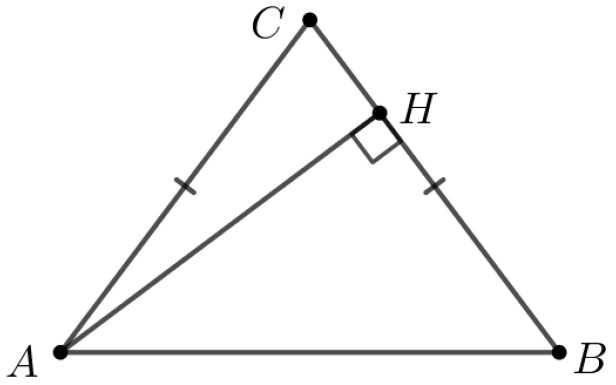
\includegraphics[align=t, width=\linewidth]{\picpath/prob_1_1}
		\end{minipage}
		%2
		\item
		\begin{minipage}[t]{\bodywidth}
			Первая цилиндрическая кружка вдвое
			выше второй, зато вторая в полтора раза
			шире. Найдите отношение объема второй
			кружки к объему первой.
			\foranswer
		\end{minipage}
		\gapwidth
		\begin{minipage}[t]{\picwidth}
			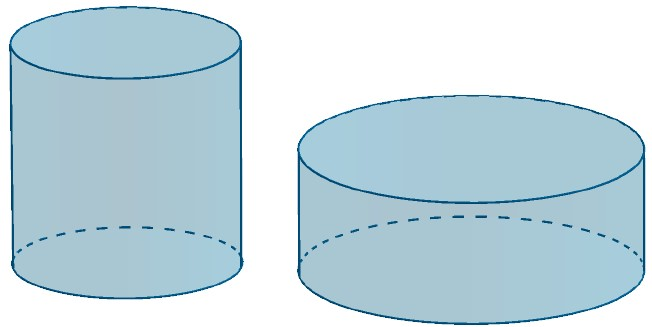
\includegraphics[align=t, width=\linewidth]{\picpath/prob_1_5}
		\end{minipage}
		%3
		\item При изготовлении подшипников диаметром \( 62 \) мм
		вероятность того, что диаметр будет отличаться от заданного
		не больше чем на \( 0, 01 \) мм, равна \( 0, 986 \).
		Найдите вероятность того, что случайно выбранный подшипник
		будет иметь диаметр меньше чем \( 61, 99 \) мм
		или больше чем \( 62, 01 \) мм.
		\foranswer
		%4
		\item Чтобы пройти в следующий круг соревнований,
		футбольной команде нужно набрать хотя бы \( 4 \) очка в двух играх.
		Если команда выигрывает, она получает \( 3 \) очка,
		в случае ничьей --- \( 1 \) очко, если проигрывает --- \( 0 \) очков.
		Найдите вероятность того, что команде удастся выйти в следующий круг соревнований.
		Считайте, что в каждой игре вероятности выигрыша и
		проигрыша одинаковы и равны \( 0,35 \).
		%5
		\item Найдите корень уравнения \( \log_7(5-3x)=3\log_72 \)
		\foranswer
	\end{listofex}
	\newpage
	\phantom{Часть 1}
	\begin{listofex}[resume]
		%6
		\item Найдите значение выражения \( \cos\dfrac{5\pi}{6}\cdot\tg\dfrac{4\pi}{3} \)
		\foranswer
		%7
		\item
		На рисунке изображён график \( y = f'(x) \)
		производной функции \( f(x) \),
		определённой на интервале \( (-5; 5) \).
		Найдите количество точек минимума функции \( f(x) \),
		принадлежащих отрезку \( [-3; 4] \).
		\begin{center}
			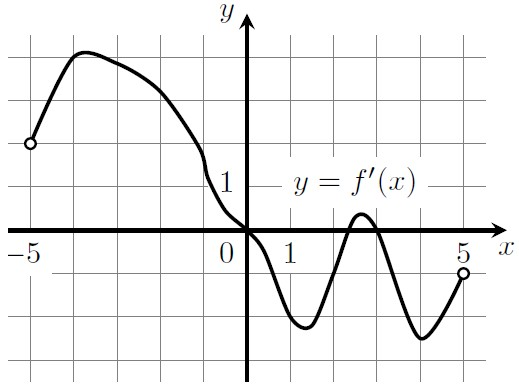
\includegraphics[align=t, width=0.5\linewidth]{\picpath/prob_1_7}
		\end{center}
		\foranswer
		%8
		\item Двигаясь со скоростью \( v = 4 \) м/с, трактор тащит сани с силой \( F = 90 \) кН,
		направленной под острым углом \( \alpha \) к горизонту.
		Мощность, развиваемая трактором, вычисляется по формуле \( N = F v \cos \alpha \).
		Найдите, при каком угле \( \alpha \) эта мощность будет равна \( 180 \) кВт.
		Ответ дайте в градусах.
		\foranswer
		%9
		\item Первая труба пропускает на \( 3 \) литра воды в минуту меньше,
		чем вторая. Сколько литров воды в минуту пропускает вторая труба,
		если резервуар объемом \( 594 \) литра она заполняет на \( 5 \) минут быстрее,
		чем первая труба заполняет резервуар объемом \( 648 \) литров?
		\foranswer
		\newpage
		\hphantom{Часть 1}
		%10
		\item 
		На рисунке изображены графики функций \( f(x) = a\sqrt{x-b}+c \) и \( g(x) = 0,75x+1 \),
		которые пересекаются в точках \( A (0;1) \) и \( B \). Найдите абсциссу точки \( B \).
		\begin{center}
			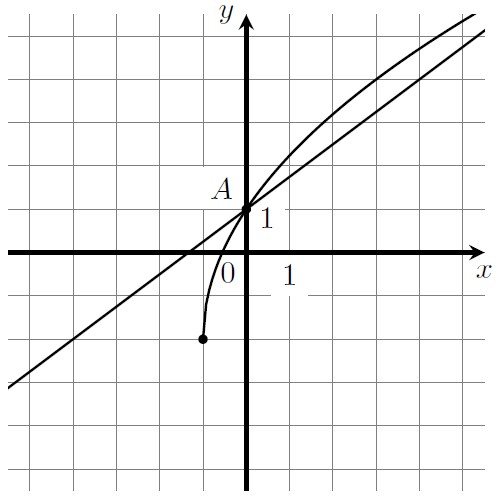
\includegraphics[align=t, width=0.45\linewidth]{\picpath/prob_1_10}
		\end{center}
		\foranswer
		%11
		\item Найдите наименьшее значение функции \( y=-x^3-27+75x \) на отрезке \( [-5;5] \).
		\foranswer
		\egepreambtwo
		\title{Часть 2}
		\egepreambthree
		%12
		\item
		а) Решите уравнение \( \sin2x + 2\cos \left( x - \dfrac{\pi}{2} \right) = \sqrt{3}\cos x + \sqrt{3} \).\\
		б) Найдите все корни этого уравнения, лежащие на отрезке \( \left[ -3\pi;-\dfrac{3\pi}{2} \right] \).
		\newpage
		\hphantom{Часть 1}
		%13
		\item
		В правильной четырехугольной призме \( ABCDA_1B_1C_1D_1 \) сторона
		основания \( AB \) равна \( 2\sqrt{3} \), а боковое ребро \( AA_1 \) равно \( 3 \).
		На ребрах \( A_1D_1 \) и \( DD_1 \) отмечены соответственно точки \( K \) и \( M \) так,
		что \( A_1K = KD_1 \), \( DM : MD_1 = 2 : 1 \).\\
		а) Докажите, что прямые \( MK \) и \( BK \) перпендикулярны.\\
		б) Найдите угол между плоскостями \( BMK \) и \( BCC_1 \).
		%14
		\item Решить неравенство:
		\[ (4^x-5\cdot2^x)^2-20\cdot(4^x-5\cdot2^x)\ge96 \]
		%15
		\item 15-го января выдан полугодовой кредит на развитие бизнеса. В таблице
		представлен график его погашения.
		\begin{center}
			\begin{tabular}{|c|c|c|c|c|c|c|c|}
				\hline
				Дата & 15.01 & 15.02 & 15.03 & 15.04 & 15.05 & 15.06 & 15.07 \\
				\hline
				Долг (в \%) & 100\% & 90\% & 80\% & 70\% & 60\% & 50\% & 0\% \\
				\hline
			\end{tabular}
		\end{center}
		В конце каждого месяца, начиная с января, текущий долг увеличивался
		на 5\%, а выплаты по погашению кредита происходили в первой половине
		каждого месяца, начиная с февраля. На сколько процентов общая сумма
		выплат при таких условиях больше суммы самого кредита?
		%16
		\item В прямоугольном треугольнике \( ABC \) с прямым углом \( C \)
		точки \( P \) и \( Q \) --- середины катетов \( AC \) и \( BC \) соответственно, \( CD \) --- высота.\\
		а) Докажите, что прямые \( PD \) и \( QD \) перпендикулярны.\\
		б) Пусть \( S \) --- точка пересечения прямых \( BC \) и \( PD \),
		а \( T \) --- точка пересечения прямых \( AC \) и \( QD \),
		причём \( AD = 6 \), \( BD = 4 \).
		Найдите площадь треугольника \( STP \).
		%17
		\item Найдите все значения параметра \( a \), при которых уравнение
		\[ x^2+4x-2|x-a|+2-a=0 \]
		имеет четыре корня.
		%18
		\item Назовем натуральное число хорошим, если в нем можно переставить
		цифры так, чтобы получившееся число делилось на \( 11 \).\\
		а) Является ли число \( 1234 \) хорошим?\\
		б) Является ли число \( 12345 \) хорошим?\\
		в) Найти наибольшее хорошее число, состоящее из различных нечетных цифр.
	\end{listofex}
\end{training}
%END_FOLD

%BEGIN_FOLD % ====>>_____ Вариант 2 _____<<====
\begin{training}[2]
	\title{Часть 1}
	\egepreambone
	\begin{listofex}
		%1
		\item
		В треугольнике со сторонами \( 9 \) и \( 6 \) проведены высоты
		к этим сторонам. Высота, проведённая к первой из этих сторон, равна \( 4 \). Чему равна высота, проведённая ко второй стороне?
		\foranswer
		%2
		\item
		\begin{minipage}[t]{\bodywidth}
			Сторона основания правильной шестиугольной
			пирамиды равна \( 3 \), боковое ребро равно \( 6 \).
			Найдите объем пирамиды.
			\foranswer
		\end{minipage}
		\gapwidth
		\begin{minipage}[t]{\picwidth}
			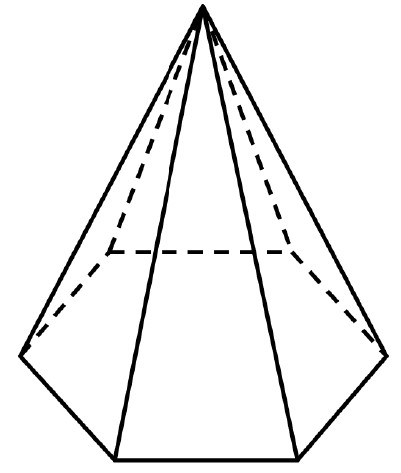
\includegraphics[align=t, width=\linewidth]{\picpath/prob_1_3}
		\end{minipage}
		%3
		\item При изготовлении подшипников диаметром \( 112 \) мм
		вероятность того, что диаметр будет отличаться от заданного
		не больше чем на \( 0, 01 \) мм, равна \( 0, 986 \).
		Найдите вероятность того, что случайно выбранный подшипник
		будет иметь диаметр меньше чем \( 111, 99 \) мм
		или больше чем \( 112, 01 \) мм.
		\foranswer
		%4
		\item Чтобы пройти в следующий круг соревнований,
		футбольной команде нужно набрать хотя бы \( 4 \) очка в двух играх.
		Если команда выигрывает, она получает \( 3 \) очка,
		в случае ничьей --- \( 1 \) очко, если проигрывает --- \( 0 \) очков.
		Найдите вероятность того, что команде удастся выйти в следующий круг соревнований.
		Считайте, что в каждой игре вероятности выигрыша и
		проигрыша одинаковы и равны \( 0,4 \).
		\foranswer
		\newpage
		\hphantom{Часть 1}
		%5
		\item Найдите корень уравнения \( \log_{1/3}(2x+6)=-2 \)
		\foranswer
		%6
		\item Найдите \( 20\cos2x \), если \( \cos x = 0,1 \)
		\foranswer
		%7
		\item 
		На рисунке изображён график \( y = f'(x) \)
		производной функции \( f(x) \),
		определённой на интервале \( (-5; 5) \).
		Найдите количество точек максимума функции \( f(x) \),
		принадлежащих отрезку \( [-3; 4] \).
		\begin{center}
			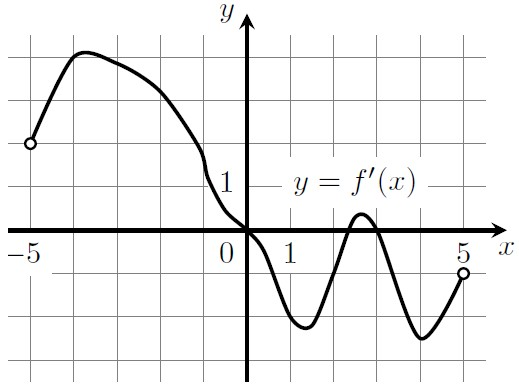
\includegraphics[align=t, width=0.5\linewidth]{\picpath/prob_1_7}
		\end{center}
		\foranswer
		%8
		\item Небольшой мячик бросают под острым углом \( \alpha \) к плоской горизонтальной поверхности земли.
		Максимальная высота полета мячика \( H \) (в м) вычисляется по формуле
		\[ H=\dfrac{v_0^2}{4g}(1-\cos2\alpha), \]
		где \( v_0 = 12 \) м/с --- начальная скорость мячика, а \( g \) --- ускорение свободного падения (считайте \( g = 10 \) м/с\( ^2 \)).
		При каком наименьшем значении угла \( \alpha \) мячик пролетит над стеной высотой \( 4,4 \) м на расстоянии \( 1 \) м?
		Ответ дайте в градусах.
		\foranswer
		\newpage
		\hphantom{Часть 1}
		%9
		\item Первый и второй насосы наполняют бассейн за \( 9 \) минут,
		второй и третий --- за \( 12 \) минут, а первый и третий --- за \( 18 \) минут.
		За сколько минут эти три насоса заполнят бассейн, работая вместе?
		\foranswer
		%10
		\item 
		На рисунке изображены графики функций \( f(x) = \frac{k}{x} \) и \( g(x) = ax+b \),
		которые пересекаются в точках \( A(-2;-3) \) и \( B \). Найдите абсциссу точки \( B \).
		\begin{center}
			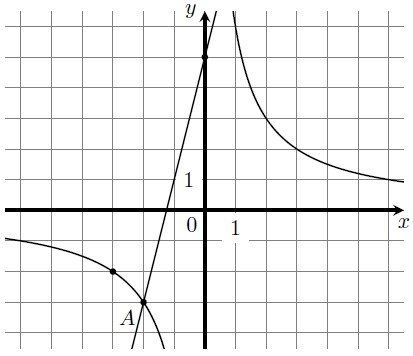
\includegraphics[align=t, width=0.45\linewidth]{\picpath/prob_1_8}
		\end{center}
		\foranswer
		%11
		\item Найдите наименьшее значение функции \( y=13+75x-x^3 \) на отрезке \( [-5;5] \).
		\foranswer
		\egepreambtwo
		\title{Часть 2}
		\egepreambthree
		%12
		\item
		а) Решите уравнение \( \sin2x - \sqrt{3} = \sqrt{3}\cos x - 2\cos \left( \dfrac{\pi}{2} - x \right) \).\\
		б) Найдите все корни этого уравнения, лежащие на отрезке \( \left[ -\pi;\dfrac{\pi}{2} \right] \).
		%13
		\item
		В правильной четырехугольной призме \( ABCDA_1B_1C_1D_1 \) сторона
		основания \( AB \) равна \( 2\sqrt{3} \), а боковое ребро \( AA_1 \) равно \( 3 \).
		На ребрах \( A_1D_1 \) и \( DD_1 \) отмечены соответственно точки \( K \) и \( M \) так,
		что \( A_1K = KD_1 \), \( DM : MD_1 = 2 : 1 \).\\
		а) Докажите, что прямые \( MK \) и \( BK \) перпендикулярны.\\
		б) Найдите угол между плоскостями \( BMK \) и \( BCC_1 \).
		%14
		\item Решить неравенство:
		\( (9^x-2\cdot3^x)^2-62\cdot(9^x-2\cdot3^x)-63\ge0 \)
		%15
		\item 15-го января выдан полугодовой кредит на развитие бизнеса. В таблице
		представлен график его погашения.
		\begin{center}
			\begin{tabular}{|c|c|c|c|c|c|c|c|}
				\hline
				Дата & 15.01 & 15.02 & 15.03 & 15.04 & 15.05 & 15.06 & 15.07 \\
				\hline
				Долг (в \%) & 100\% & 90\% & 80\% & 70\% & 60\% & 50\% & 0\% \\
				\hline
			\end{tabular}
		\end{center}
		В конце каждого месяца, начиная с января, текущий долг увеличивался
		на 5\%, а выплаты по погашению кредита происходили в первой половине
		каждого месяца, начиная с февраля. На сколько процентов общая сумма
		выплат при таких условиях больше суммы самого кредита?
		%16
		\item В прямоугольном треугольнике \( ABC \) с прямым углом \( C \)
		точки \( P \) и \( Q \) --- середины катетов \( AC \) и \( BC \) соответственно, \( CD \) --- высота.\\
		а) Докажите, что прямые \( PD \) и \( QD \) перпендикулярны.\\
		б) Пусть \( S \) --- точка пересечения прямых \( BC \) и \( PD \),
		а \( T \) --- точка пересечения прямых \( AC \) и \( QD \),
		причём \( AD = 6 \), \( BD = 4 \).
		Найдите площадь треугольника \( STP \).
		%17
		\item Найдите все значения параметра \( a \), при которых уравнение
		\[ x^2+4x-2|x-a|+2-a=0 \]
		имеет четыре корня.
		%18
		\item Назовем натуральное число хорошим, если в нем можно переставить
		цифры так, чтобы получившееся число делилось на \( 11 \).\\
		а) Является ли число \( 1234 \) хорошим?\\
		б) Является ли число \( 12345 \) хорошим?\\
		в) Найти наибольшее хорошее число, состоящее из различных нечетных цифр.
	\end{listofex}
\end{training}
%END_FOLD

%BEGIN_FOLD % ====>>_____ Вариант 3 _____<<====
\begin{training}[3]
	\title{Часть 1}
	\egepreambone
	\begin{listofex}
		%1
		\item
		\begin{minipage}[t]{\bodywidth}
			Площадь параллелограмма \( ABCD \) равна \( 2 \)4.
			Точка \( M \) --- середина стороны \( BC \).
			Найдите площадь трапеции \( AMCD \).
			\foranswer
		\end{minipage}
		\gapwidth
		\begin{minipage}[t]{\picwidth}
			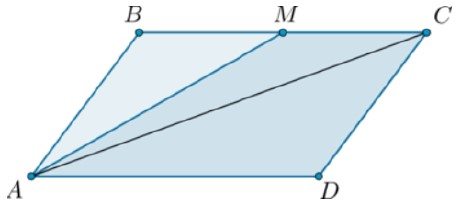
\includegraphics[align=t, width=\linewidth]{\picpath/prob_1_2}
		\end{minipage}
		%2
		\item
		\begin{minipage}[t]{\bodywidth}
			Объём треугольной призмы,
			отсекаемой от куба плоскостью, проходящей через
			середины двух рёбер, выходящих из одной
			вершины, и параллельной третьему ребру,
			выходящему из этой же вершины, равен \( 4 \).
			Найдите объём куба.
			\foranswer
		\end{minipage}
		\gapwidth
		\begin{minipage}[t]{\picwidth}
			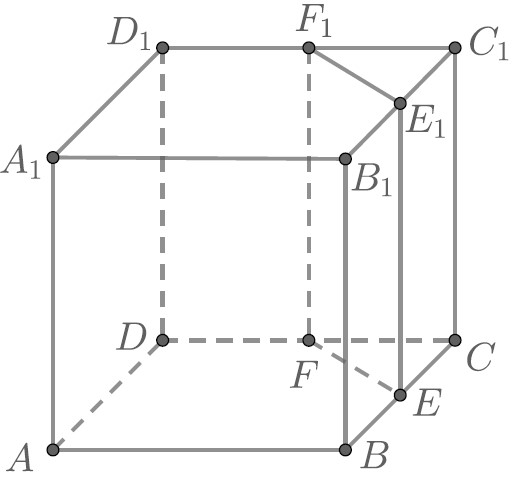
\includegraphics[align=t, width=\linewidth]{\picpath/prob_1_4}
		\end{minipage}
		%3
		\item Вероятность того, что новый принтер в течение года поступит в гарантийный ремонт, равна \( 0, 097 \).
		В некотором городе из \( 1000 \) проданных принтеров в течение года в мастерские по гарантии поступила \( 101 \) штука.
		На сколько отличается частота события «принтер поступил в гарантийный ремонт» от вероятности этого события?
		\foranswer
		%4
		\item Чтобы пройти в следующий круг соревнований,
		футбольной команде нужно набрать хотя бы \( 4 \) очка в двух играх.
		Если команда выигрывает, она получает \( 3 \) очка,
		в случае ничьей --- \( 1 \) очко, если проигрывает --- \( 0 \) очков.
		Найдите вероятность того, что команде удастся выйти в следующий круг соревнований.
		Считайте, что в каждой игре вероятности выигрыша и
		проигрыша одинаковы и равны \( 0,45 \).
		\foranswer
		\newpage
		\hphantom{Часть 1}
		%5
		\item Найдите корень уравнения \( \log_{1/4}(2x+6)=-2 \)
		\foranswer
		%6
		\item Найдите значение выражения
		\( 7\sqrt{2}\cdot\sin\dfrac{15\pi}{8}\cdot\cos\dfrac{15\pi}{8} \)
		\foranswer
		%7
		\item 
		На рисунке изображён график функции \( y = f(x) \), определённой на
		интервале \( (-9; 2) \). Определите количество целых точек, в которых производная функции отрицательна.
		\begin{center}
			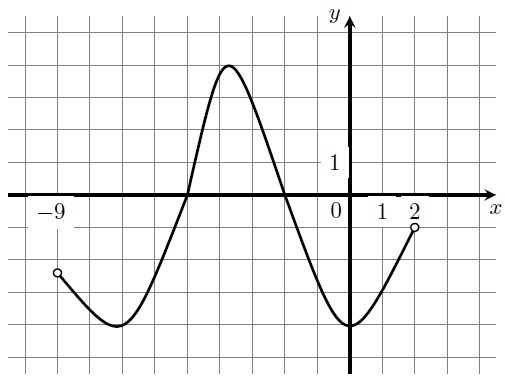
\includegraphics[align=t, width=0.5\linewidth]{\picpath/prob_1_6}
		\end{center}
		\foranswer
		%8
		\item Скорость тела, движущегося прямолинейно, вычисляется по формуле
		\[ v(t) = -t^2+7,4t-7, \]
		где \( t \) --- время (в секундах), прошедшее с момента начала движения,
		\( v(t) \) --- скорость в соответствующий момент времени.
		Сколько секунд скорость тела будет не менее \( 5 \) м/с?
		\foranswer
		%9
		\item Первая труба пропускает на \( 1 \) литр воды в минуту меньше, чем вторая.
		Сколько литров воды в минуту пропускает первая труба, если резервуар объемом \( 110 \) литров она заполняет на \( 2 \) минуты дольше,
		чем вторая труба заполняет резервуар объемом \( 99 \) литров?
		\foranswer
		\newpage
		\hphantom{Часть 1}
		%10
		\item 
		На рисунке изображены графики функций \( f(x) = \dfrac{x^2}{a}+bx+c \), где числа
		\( a \), \( b \), \( c \) --- целые. Найдите \( f(3,5) \).
		\begin{center}
			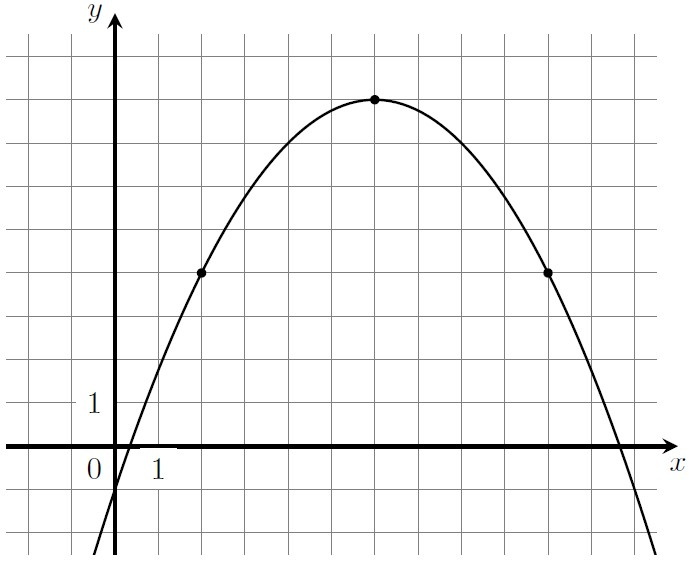
\includegraphics[align=t, width=0.5\linewidth]{\picpath/prob_1_9}
		\end{center}
		\foranswer
		%11
		\item Найдите точку минимума функции \( y=x\sqrt{x}-1,5\ln x + 2 \).
		\foranswer
		\egepreambtwo
		\title{Часть 2}
		\egepreambthree
		%12
		\item
		а) Решите уравнение \( \sin2x + 2\cos \left( x - \dfrac{\pi}{2} \right) = \sqrt{3}\cos x + \sqrt{3} \).\\
		б) Найдите все корни этого уравнения, лежащие на отрезке \( \left[ 2\pi;\dfrac{5\pi}{2} \right] \).
		\item
		В правильной четырехугольной призме \( ABCDA_1B_1C_1D_1 \) сторона
		основания \( AB \) равна \( 2\sqrt{3} \), а боковое ребро \( AA_1 \) равно \( 3 \).
		На ребрах \( A_1D_1 \) и \( DD_1 \) отмечены соответственно точки \( K \) и \( M \) так,
		что \( A_1K = KD_1 \), \( DM : MD_1 = 2 : 1 \).\\
		а) Докажите, что прямые \( MK \) и \( BK \) перпендикулярны.\\
		б) Найдите угол между плоскостями \( BMK \) и \( BCC_1 \).
		%14
		\item Решить неравенство:
		\[ (4^x-5\cdot2^x)^2-96\ge20\cdot(4^x-5\cdot2^x) \]
		%15
		\item 15-го января выдан полугодовой кредит на развитие бизнеса. В таблице
		представлен график его погашения.
		\begin{center}
			\begin{tabular}{|c|c|c|c|c|c|c|c|}
				\hline
				Дата & 15.01 & 15.02 & 15.03 & 15.04 & 15.05 & 15.06 & 15.07 \\
				\hline
				Долг (в \%) & 100\% & 90\% & 80\% & 70\% & 60\% & 50\% & 0\% \\
				\hline
			\end{tabular}
		\end{center}
		В конце каждого месяца, начиная с января, текущий долг увеличивался
		на 5\%, а выплаты по погашению кредита происходили в первой половине
		каждого месяца, начиная с февраля. На сколько процентов общая сумма
		выплат при таких условиях больше суммы самого кредита?
		%16
		\item В прямоугольном треугольнике \( ABC \) с прямым углом \( C \)
		точки \( P \) и \( Q \) --- середины катетов \( AC \) и \( BC \) соответственно, \( CD \) --- высота.\\
		а) Докажите, что прямые \( PD \) и \( QD \) перпендикулярны.\\
		б) Пусть \( S \) --- точка пересечения прямых \( BC \) и \( PD \),
		а \( T \) --- точка пересечения прямых \( AC \) и \( QD \),
		причём \( AD = 6 \), \( BD = 4 \).
		Найдите площадь треугольника \( STP \).
		%17
		\item Найдите все значения параметра \( a \), при которых уравнение
		\[ x^2+4x-2|x-a|+2-a=0 \]
		имеет четыре корня.
		%18
		\item Назовем натуральное число хорошим, если в нем можно переставить
		цифры так, чтобы получившееся число делилось на \( 11 \).\\
		а) Является ли число \( 1234 \) хорошим?\\
		б) Является ли число \( 12345 \) хорошим?\\
		в) Найти наибольшее хорошее число, состоящее из различных нечетных цифр.
	\end{listofex}
\end{training}
%END_FOLD